% ch3p7_003: Naming nodes
% using parentheses, liberal with order
\documentclass[tikz, border=10pt]{standalone}

\usepackage{tikz}
\usetikzlibrary{arrows.meta, decorations.pathmorphing, backgrounds, positioning, fit, petri}

\begin{document}
	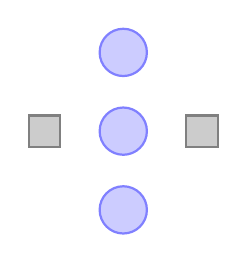
\begin{tikzpicture}[
		%inner sep=2mm,
		place/.style={circle, draw=blue!50, fill=blue!20, thick, inner sep=0pt, minimum size=6mm},
		transition/.style={rectangle, draw=black!50, fill=black!20, thick, inner sep=0pt, minimum size=4mm}
		]
		\node [place] (waiting 1) at (0, 2) {};
		\node [place] (critical 1) at (0, 1) {};
		\node [place] (semaphore) at (0, 0) {};
		\node [transition] (leave critical) at (1, 1) {};
		\node [transition] (enter critical) at (-1, 1) {};
	\end{tikzpicture}
\end{document}